\documentclass[../masters.tex]{subfiles}

\begin{document}
\graphicspath{{./imgs/}{../imgs/}} %look for images

\section{CSTR Model}
In this section we introduce the model we will use to illustrate the techniques we develop in this dissertation. The model is a simple continuously stirred tank reactor (CSTR) undergoing an exothermic, irreversible first order reaction where $A \rightarrow B$. A schematic diagram of the reactor is shown in Figure \ref{fig_cstr_diagram}. The model is taken from literature \cite{cstrmodel}.
\begin{figure}[H] 
\centering
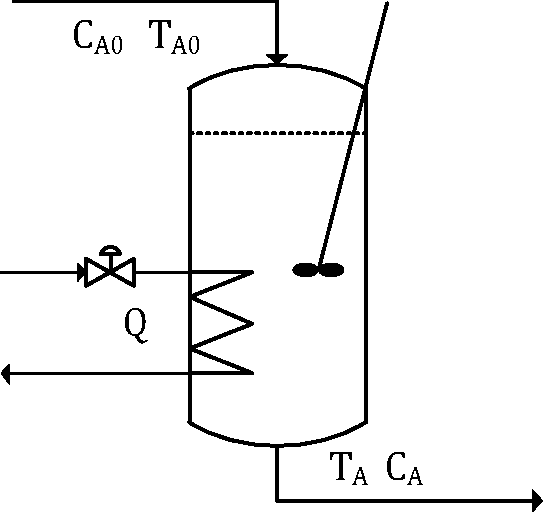
\includegraphics[scale=0.8]{cstr_diagram.pdf}
\caption{Diagram of a simple CSTR}
\label{fig_cstr_diagram}
\end{figure}
The state space equations describing the reactor are shown in (\ref{eq_cstrmodel}) with parameters shown in ().
\begin{equation}
\begin{aligned}
C
\end{aligned}
\label{eq_cstrmodel}
\end{equation}



\bibliographystyle{plain}
\bibliography{research}

\end{document}